\begin{framed}\noindent
	
	\textbf{Bài 1 - Bài toán đề nghị tháng 8/2018 - Nguyễn Duy Khương}
	
	Cho tam giác $\triangle ABC$ có tiếp điểm đường tròn bàng tiếp góc $\angle A$ với $BC$ là $E$. Gọi $K$ là hình chiếu của $E$ lên đường trung bình ứng với đỉnh $A$ của tam giác $\triangle ABC$. Chứng minh $(K, KE)$ tiếp xúc với $(O)$.

	
\end{framed}

\begin{center}
	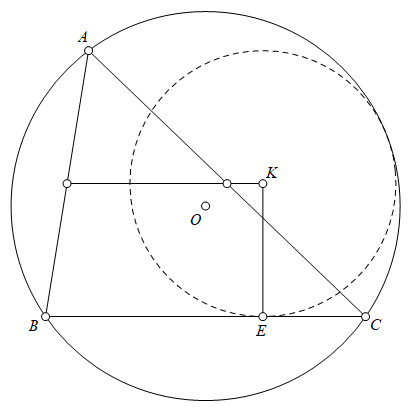
\includegraphics[scale=0.5]{T082018/T82018_KhuongNguyen}
	
\end{center}

\begin{framed}\noindent
	
	\textbf{Bài 2 - Bài toán đề nghị tháng 8/2018 - Nguyễn Hoàng Nam}
	
	Cho tam giác $\triangle ABC$ nội tiếp $(O)$. Trung trực $AB$ cắt đường tròn \textit{A-Apollonius} \footnotemark tại $H, I$ ($I$ gần $O$ hơn $H$). $K$ đối xứng với $I$ qua $BC$. Gọi $J = AK \cap CH$. Chứng minh rằng $JK$ là phân giác góc $\angle BJC$.
	
\end{framed}

\footnotetext{Đường tròn $A-Apollonius$ của tam giác $\triangle ABC$ là đường tròn đi qua đỉnh $A$ và chân 2 đường phân giác của góc $\angle BAC$.}

\begin{center}
	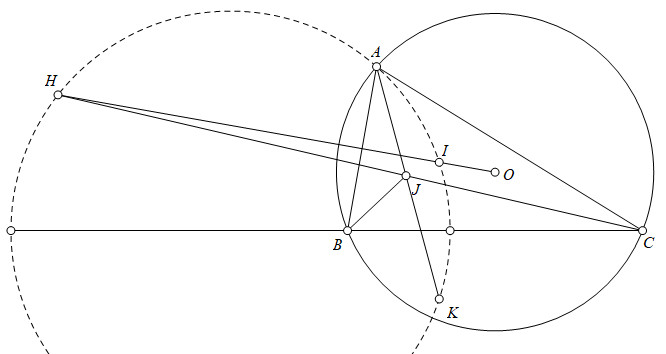
\includegraphics[scale=0.5]{T082018/T82018_NamNH}
	
\end{center}

\begin{framed}\noindent
	
	\textbf{Bài 3 - Bài toán đề nghị tháng 8/2018 - Phan Quang Trí}
	
	Cho tam giác $\triangle ABC$ nội tiếp đường tròn $(O)$. Gọi $X, Y$ lần lượt là trung điểm $CA, AB$. Gọi $K = AO \cap BC$. Gọi $E, F$ lần lượt là tâm của $(AXK), (AYK)$. Chứng minh $YE, XF$ cắt nhau trên tiếp tuyến tại $A$ của $(O)$.
	
\end{framed}

\begin{center}
	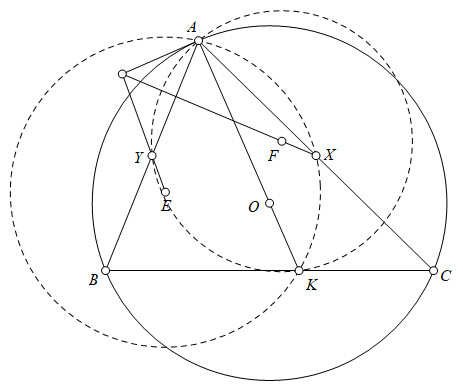
\includegraphics[scale=0.5]{T082018/T82018_TriPQ}
	
\end{center}